%% This is an example first chapter.  You should put chapter/appendix that you
%% write into a separate file, and add a line \include{yourfilename} to
%% main.tex, where `yourfilename.tex' is the name of the chapter/appendix file.
%% You can process specific files by typing their names in at the 
%% \files=
%% prompt when you run the file main.tex through LaTeX.
\chapter{Introduction}

\section{The SM Higgs mechanism}

\section{The Glashow-Weinberg-Salam theory of Weak interactions}

\section{The W,Z, and Higgs boson production at the LHC}

\section{Extended Higgs Sector and MSSM}

\section{Monte Carlo Simulations and Cross Sections}
    
\section{The Large Hadron Collider}
The Large Hadron Collider (LHC)\cite{1748-0221-3-08-S08001} is a $26.7$ km circular collider designed to collide beams of protons at centre-of-mass energies up to 14 \TeV. Figure~\ref{fig:cern} shows the schematic representation of the accelerator complex at CERN. 

\begin{figure}[h]
\centering
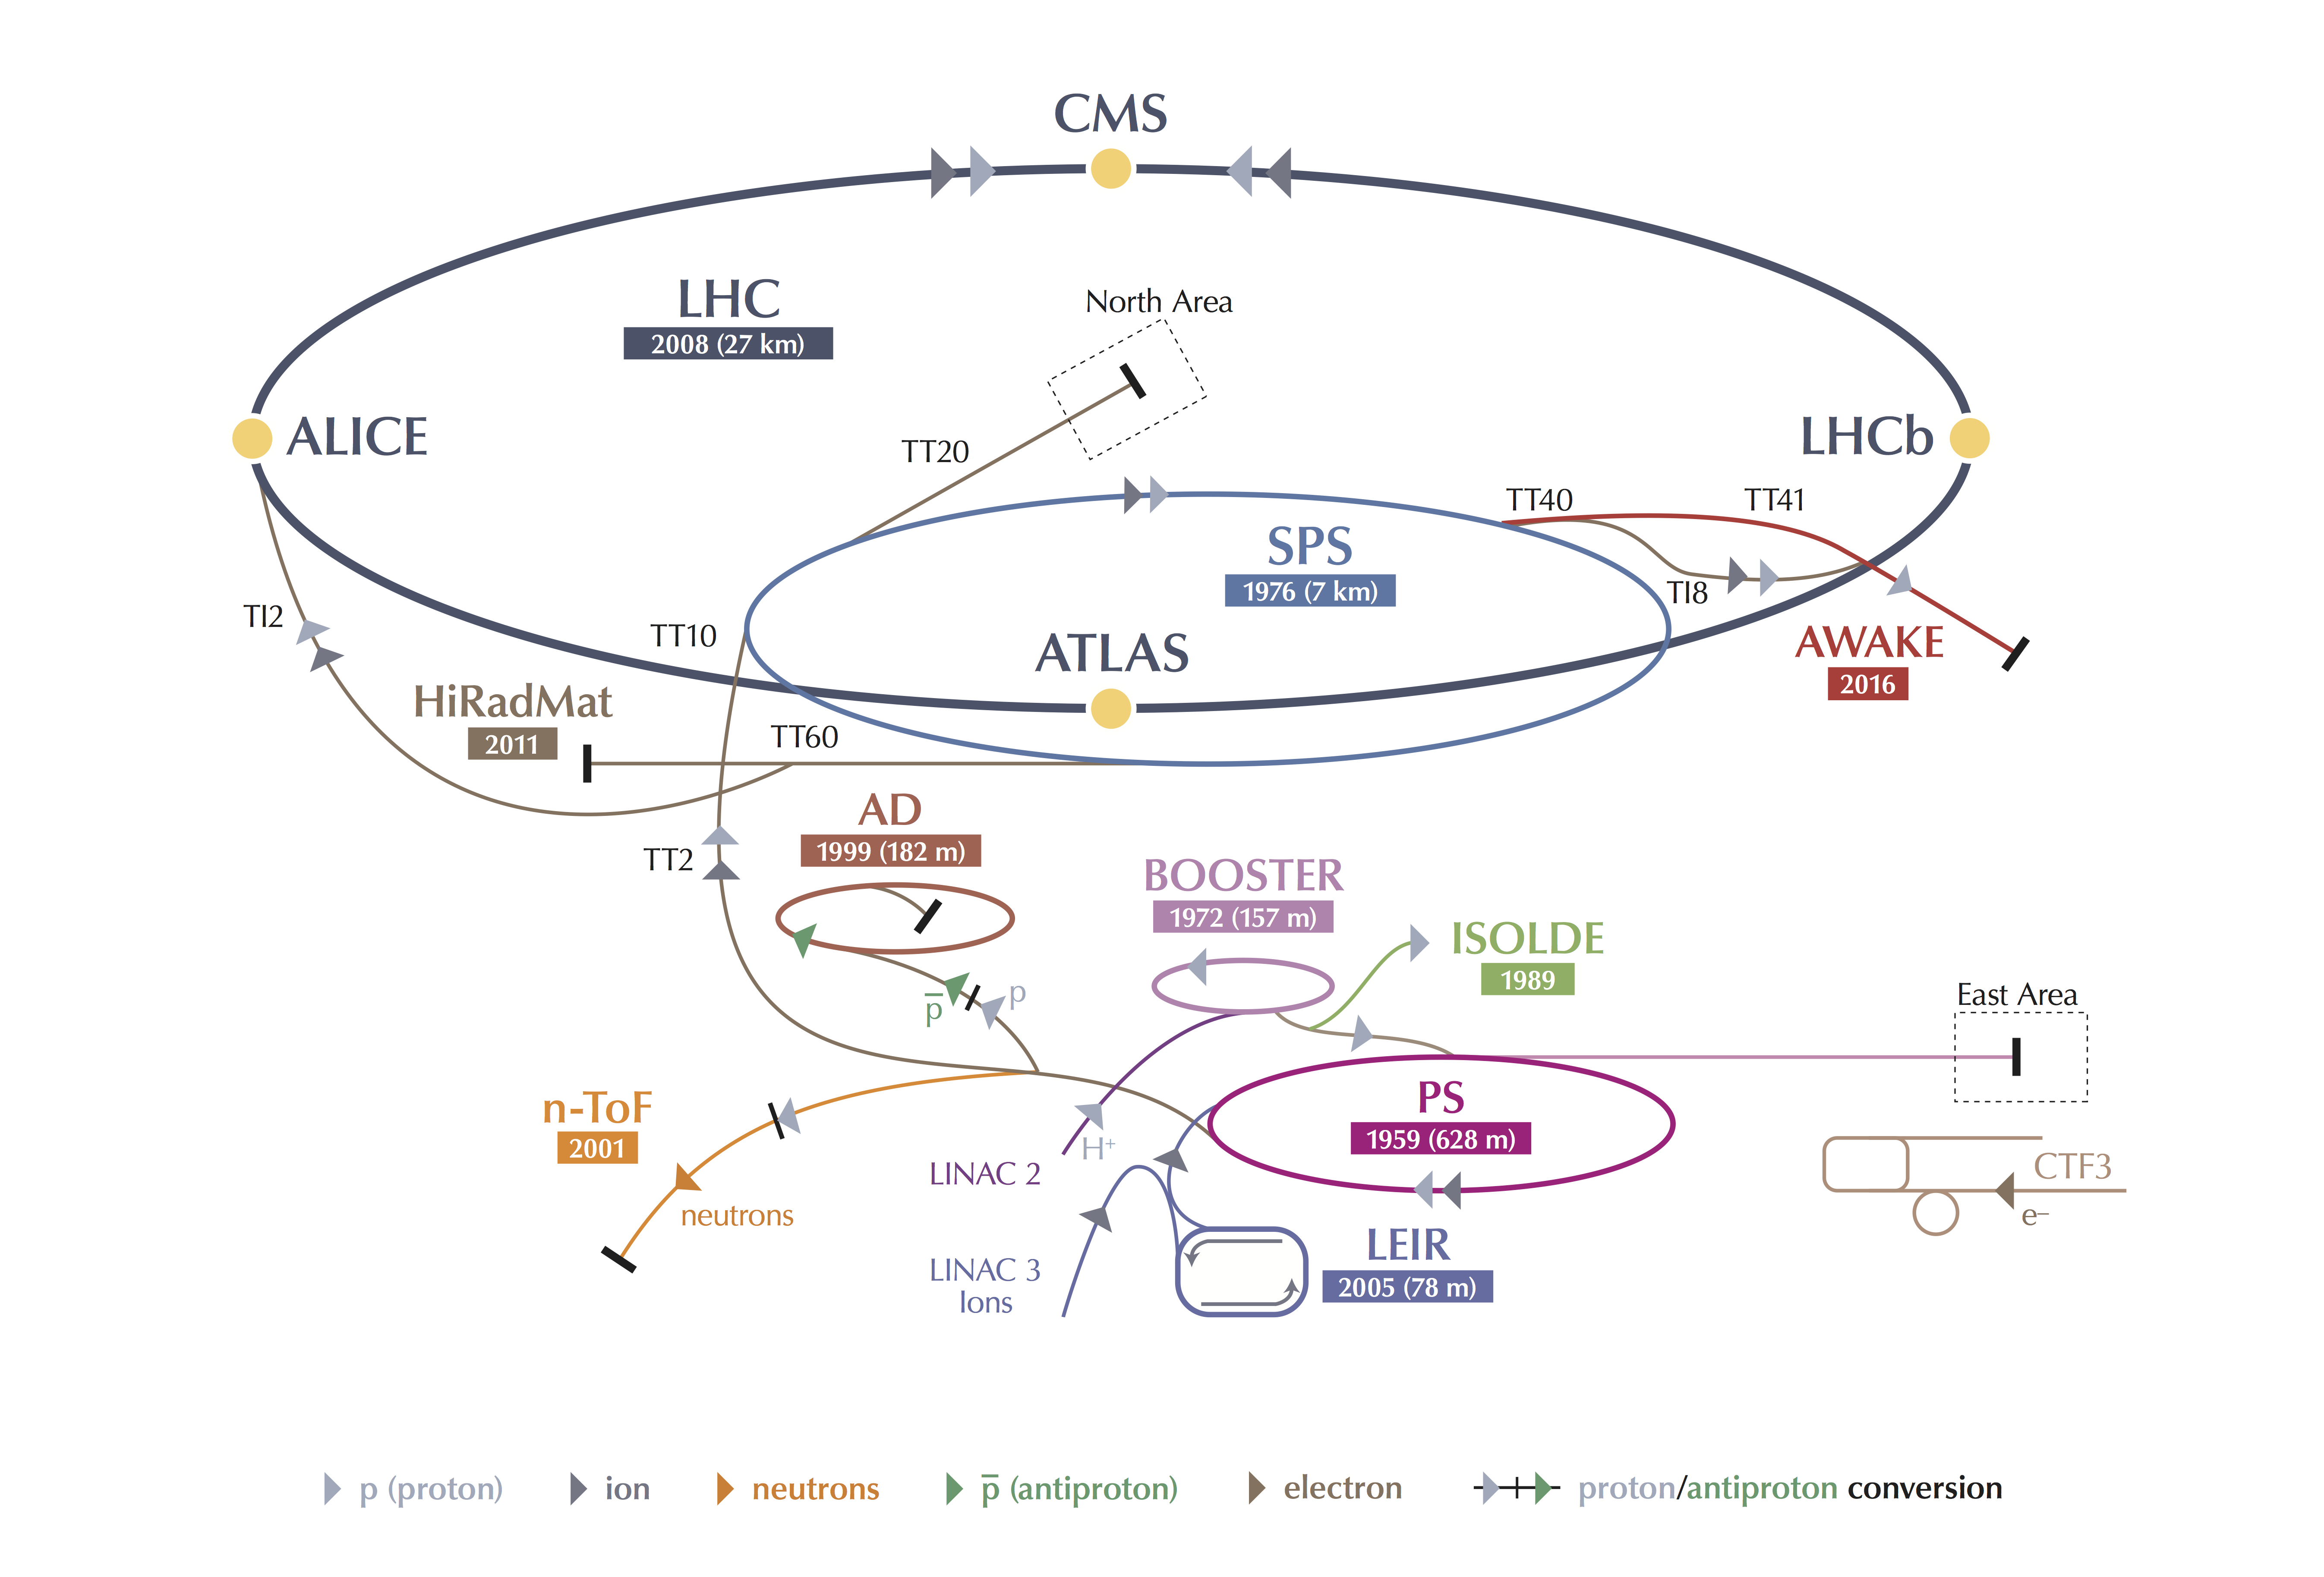
\includegraphics[width=1.0\textwidth]{figures_chapter2/cern_complex.jpg}
\caption{A schematic representation of the CERN accelerator complex\cite{Haffner:1621894}.}
\label{fig:cern}
\end{figure}


%\subsection{Post Multiply Normalization}


